\documentclass[tikz,border=8pt]{standalone}
\usepackage{amsmath,amssymb}
\usetikzlibrary{arrows.meta,calc}

\begin{document}
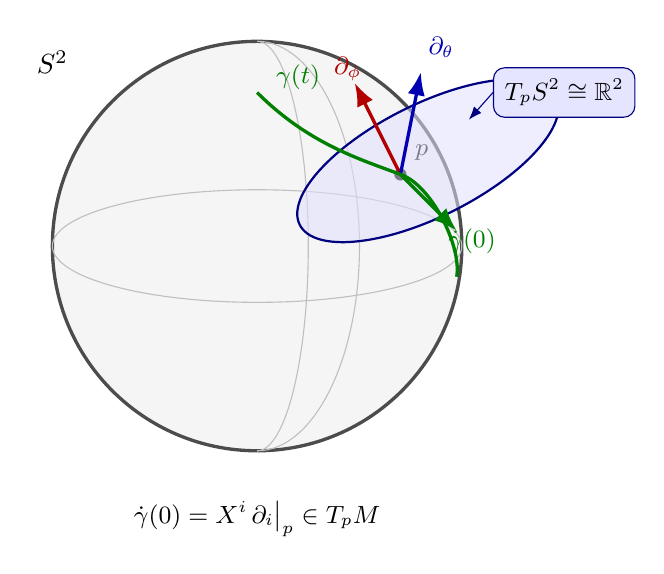
\begin{tikzpicture}[>=Latex, scale=1.3]

  % Sphere
  \draw[very thick, gray!60!black, fill=gray!8] (0, 0) circle (2.0);
  % equator
  \draw[gray!50, thin] (0, 0) ellipse (2.0 and 0.55);
  % a couple of meridians (front)
  \draw[gray!50, thin] (0, 2) arc (90:-90:0.5 and 2);
  \draw[gray!50, thin] (0, 2) arc (90:-90:1.0 and 2);

  % point p on sphere
  \pgfmathsetmacro{\px}{1.4}
  \pgfmathsetmacro{\py}{0.7}
  \fill[black] (\px, \py) circle (0.06);
  \node[font=\small, anchor=south west] at (\px+0.05, \py+0.04) {$p$};

  % normal direction at p
  \pgfmathsetmacro{\nrm}{sqrt(\px*\px+\py*\py)}
  \pgfmathsetmacro{\nx}{\px/\nrm}
  \pgfmathsetmacro{\ny}{\py/\nrm}

  % tangent plane (slanted ellipse outside sphere)
  \pgfmathsetmacro{\angtan}{atan2(\ny,\nx)}
  \pgfmathsetmacro{\cx}{\px+\nx*0.3}
  \pgfmathsetmacro{\cy}{\py+\ny*0.3}
  \filldraw[blue!50!black, fill=blue!12, fill opacity=0.55, thick]
    (\cx, \cy) ellipse [x radius=1.4, y radius=0.55, rotate=\angtan];

  % basis vectors at p (∂_φ in tangent direction perpendicular to normal in plane;
  % we draw it along the slanted-ellipse major axis direction)
  \pgfmathsetmacro{\tx}{-\ny}
  \pgfmathsetmacro{\ty}{\nx}
  \draw[->, very thick, red!70!black] (\px, \py) -- ($(\px,\py)+(\tx*1.0, \ty*1.0)$);
  \node[font=\small, red!70!black] at ($(\px,\py)+(\tx*1.15, \ty*1.15)$) {$\partial_\phi$};

  % ∂_θ (vertical-ish direction)
  \draw[->, very thick, blue!70!black] (\px, \py) -- ($(\px,\py)+(0.2, 1.0)$);
  \node[font=\small, blue!70!black, anchor=south west] at ($(\px,\py)+(0.18, 1.05)$) {$\partial_\theta$};

  % curve gamma through p
  \draw[very thick, green!50!black, smooth]
    (0.0, 1.5) .. controls (0.5, 1.0) and (1.0, 0.85) .. (\px, \py)
    .. controls (1.7, 0.6) and (2.0, 0.0) .. (1.95, -0.3);
  \node[font=\small, green!50!black] at (0.4, 1.65) {$\gamma(t)$};

  % velocity \dot\gamma(0) at p
  \draw[->, very thick, green!50!black] (\px, \py) -- ($(\px,\py)+(0.55, -0.55)$);
  \node[font=\small, green!50!black] at ($(\px,\py)+(0.7, -0.65)$) {$\dot\gamma(0)$};

  % S^2 label
  \node[font=\bfseries] at (-2.0, 1.8) {$S^2$};

  % Tangent space label box
  \node[font=\small, fill=blue!10, draw=blue!50!black, rounded corners, inner sep=4pt] (TS) at (3.0, 1.5)
    {$T_pS^2 \cong \mathbb R^2$};
  \draw[->, thin, blue!50!black] (TS.west) -- (\cx+0.4, \cy+0.4);

  % bottom equation
  \node[font=\small, anchor=north] at (0, -2.4)
    {$\dot\gamma(0)=X^i\,\partial_i\big|_p \in T_p M$};
\end{tikzpicture}
\end{document}
